% -*- TeX-engine: xetex; eval: (auto-fill-mode 0); eval: (visual-line-mode 1); -*-
% Compile with XeLaTeX

%%%%%%%%%%%%%%%%%%%%%%%
% Option 1: Slides: (comment for handouts)   %
%%%%%%%%%%%%%%%%%%%%%%%

%\documentclass[slidestop,compress,mathserif,12pt,t,professionalfonts,xcolor=table]{beamer}
%
%% solution stuff
%\newcommand{\solnMult}[1]{
%\only<1>{#1}
%\only<2->{\red{\textbf{#1}}}
%}
%\newcommand{\soln}[1]{\textit{#1}}

%%%%%%%%%%%%%%%%%%%%%%%%%%%%%%%
% Option 2: Handouts, without solutions (post before class)    %
%%%%%%%%%%%%%%%%%%%%%%%%%%%%%%%

 \documentclass[11pt,containsverbatim,handout,xcolor=xelatex,dvipsnames,table]{beamer}

 % handout layout
 \usepackage{pgfpages}
 \pgfpagesuselayout{4 on 1}[letterpaper,landscape,border shrink=5mm]

 % solution stuff
 \newcommand{\solnMult}[1]{#1}
 \newcommand{\soln}[1]{}

%%%%%%%%%%%%%%%%%%%%%%%%%%%%%%%%%%%%
% Option 3: Handouts, with solutions (may post after class if need be)    %
%%%%%%%%%%%%%%%%%%%%%%%%%%%%%%%%%%%%

% \documentclass[11pt,containsverbatim,handout,xcolor=xelatex,dvipsnames,table]{beamer}

% % handout layout
% \usepackage{pgfpages}
% \pgfpagesuselayout{4 on 1}[letterpaper,landscape,border shrink=5mm]

% % solution stuff
% \newcommand{\solnMult}[1]{\red{\textbf{#1}}}
% \newcommand{\soln}[1]{\textit{#1}}

%%%%%%%%%%%%%%%%%%%%%%%%%%%%%%%
% Option 4: Notes Only
%%%%%%%%%%%%%%%%%%%%%%%%%%%%%%%

% % See http://tex.stackexchange.com/questions/114219/add-notes-to-latex-beamer
% \documentclass[10pt,containsverbatim,xcolor=xelatex,dvipsnames,table,notes=only]{beamer}

% % handout layout
% \usepackage{pgfpages}
% \pgfpagesuselayout{2 on 1}[letterpaper, landscape, border shrink=5mm]

% % solution stuff
% \newcommand{\solnMult}[1]{#1}
% \newcommand{\soln}[1]{}

%%%%%%%%%%
% Load style file, defaults  %
%%%%%%%%%%

%%%%%%%%%%%%%%%%
% Themes
%%%%%%%%%%%%%%%%

% See http://deic.uab.es/~iblanes/beamer_gallery/ for mor options

% Style theme
\usetheme{Pittsburgh}

% Color theme
\usecolortheme{seahorse}

% Helvetica Neue Light for most text
\usepackage{fontspec}
\setsansfont{Helvetica Neue Light}

%%%%%%%%%%%%%%%%
% Packages
%%%%%%%%%%%%%%%%

\usepackage{geometry}
\usepackage{graphicx}
\usepackage{amssymb}
\usepackage{epstopdf}
\usepackage{amsmath}  	% this permits text in eqnarray among other benefits
\usepackage{url}		% produces hyperlinks
\usepackage[english]{babel}
\usepackage{colortbl}	% allows for color usage in tables
\usepackage{multirow}	% allows for rows that span multiple rows in tables
\usepackage{color}		% this package has a variety of color options
\usepackage{pgf}
\usepackage{calc}
\usepackage{ulem}
\usepackage{multicol}
\usepackage{textcomp}
\usepackage{listings}
\usepackage{changepage}
\usepackage{tikz}
\usetikzlibrary{trees}		% for probability trees
\usepackage{fancyvrb}	% for colored code chunks
\usepackage{nameref}

%%%%%%%%%%%%%%%%
% Remove navigation symbols
%%%%%%%%%%%%%%%%

\beamertemplatenavigationsymbolsempty
\hypersetup{pdfpagemode=UseNone} % don't show bookmarks on initial view

%%%%%%%%%%%%%%%%
% User defined colors
%%%%%%%%%%%%%%%%

% Pantone 2015 Spring colors
% http://iwork3.us/2014/09/16/pantone-2015-spring-fashion-report/
% update each semester or year

\xdefinecolor{custom_blue}{rgb}{0, 0.70, 0.79} % scuba blue
\xdefinecolor{custom_darkBlue}{rgb}{0.11, 0.31, 0.54} % classic blue
\xdefinecolor{custom_orange}{rgb}{0.97, 0.57, 0.34} % tangerine
\xdefinecolor{custom_green}{rgb}{0.49, 0.81, 0.71} % lucite green
\xdefinecolor{custom_red}{rgb}{0.58, 0.32, 0.32} % marsala

\xdefinecolor{custom_lightGray}{rgb}{0.78, 0.80, 0.80} % glacier gray
\xdefinecolor{custom_darkGray}{rgb}{0.54, 0.52, 0.53} % titanium

%%%%%%%%%%%%%%%%
% Template colors
%%%%%%%%%%%%%%%%

\setbeamercolor*{palette primary}{fg=white,bg= custom_blue}
\setbeamercolor*{palette secondary}{fg=black,bg= custom_blue!80!black}
\setbeamercolor*{palette tertiary}{fg=white,bg= custom_blue!80!black!80}
\setbeamercolor*{palette quaternary}{fg=white,bg= custom_blue}

\setbeamercolor{structure}{fg= custom_blue}
\setbeamercolor{frametitle}{bg= custom_blue!90}
\setbeamertemplate{blocks}[shadow=false]
\setbeamersize{text margin left=2em,text margin right=2em}

%%%%%%%%%%%%%%%%
% Styling fonts, bullets, etc.
%%%%%%%%%%%%%%%%

% title slide
\setbeamerfont{title}{size=\large,series=\bfseries}
\setbeamerfont{subtitle}{size=\large,series=\mdseries}
%\setbeamerfont{institute}{size=\large,series=\mdseries}

% color of alerted text
\setbeamercolor{alerted text}{fg=custom_orange}

% styling of itemize bullets
\setbeamercolor{item}{fg=custom_blue}
\setbeamertemplate{itemize item}{{{\small$\blacktriangleright$}}}
\setbeamercolor{subitem}{fg=custom_blue}
\setbeamertemplate{itemize subitem}{{\textendash}}
\setbeamerfont{itemize/enumerate subbody}{size=\footnotesize}
\setbeamerfont{itemize/enumerate subitem}{size=\footnotesize}

% styling of enumerate bullets
\setbeamertemplate{enumerate item}{\insertenumlabel.}
\setbeamerfont{enumerate item}{family={\fontspec{Helvetica Neue}}}
\setbeamerfont{enumerate subitem}{family={\fontspec{Helvetica Neue}}}
\setbeamerfont{enumerate subsubitem}{family={\fontspec{Helvetica Neue}}}

% make frame titles small to make room in the slide
\setbeamerfont{frametitle}{size=\small} 

% set Helvetica Neue font for frame and section titles
\setbeamerfont{frametitle}{family={\fontspec{Helvetica Neue}}}
\setbeamerfont{sectiontitle}{family={\fontspec{Helvetica Neue}}}
\setbeamerfont{section in toc}{family={\fontspec{Helvetica Neue}}}
\setbeamerfont{subsection in toc}{family={\fontspec{Helvetica Neue}}, size=\small}
\setbeamerfont{footline}{family={\fontspec{Helvetica Neue}}}
\setbeamerfont{subsection in toc}{family={\fontspec{Helvetica Neue}}}
\setbeamerfont{block title}{family={\fontspec{Helvetica Neue}}}

%%%%%%%%%%%%%%%%
% New fonts accessed by fontspec package
%%%%%%%%%%%%%%%%

% Monaco font for code
\newfontfamily{\monaco}{Monaco}

%%%%%%%%%%%%%%%%
% Color text commands
%%%%%%%%%%%%%%%%

%orange
\newcommand{\orange}[1]{\textit{\textcolor{custom_orange}{#1}}}

% yellow
\newcommand{\yellow}[1]{\textit{\textcolor{yellow}{#1}}}

% blue
\newcommand{\blue}[1]{\textit{\textcolor{blue}{#1}}}

% green
\newcommand{\green}[1]{\textit{\textcolor{custom_green}{#1}}}

% red
\newcommand{\red}[1]{\textit{\textcolor{custom_red}{#1}}}

% dark gray
\newcommand{\darkgray}[1]{\textit{\textcolor{custom_darkGray}{#1}}}

% light gray
\newcommand{\lightgray}[1]{\textit{\textcolor{custom_lightGray}{#1}}}

% pink
\newcommand{\pink}[1]{\textit{\textcolor{pink}{#1}}}


%%%%%%%%%%%%%%%%
% Custom commands
%%%%%%%%%%%%%%%%

% empty box for probability tree frame
\newcommand{\emptybox}[2]{
	\fbox{ \begin{minipage}{#1} \hfill\vspace{#2} \end{minipage} }
}

% cancel
\newcommand{\cancel}[1]{%
    \tikz[baseline=(tocancel.base)]{
        \node[inner sep=0pt,outer sep=0pt] (tocancel) {#1};
        \draw[red, line width=0.5mm] (tocancel.south west) -- (tocancel.north east);
    }%
}

% degree
\newcommand{\degree}{\ensuremath{^\circ}}

% cite
\newcommand{\ct}[1]{
\vfill
{\tiny #1}}

% Note
\newcommand{\Note}[1]{
\rule{2.5cm}{0.25pt} \\ \textit{\footnotesize{\textcolor{custom_red}{Note:} \textcolor{custom_darkGray}{#1}}}}

% Remember
\newcommand{\Remember}[1]{\textit{\scriptsize{\textcolor{custom_red}{Remember:} #1}}}

% links: webURL, webLink
\newcommand{\webURL}[1]{\urlstyle{same}{\textit{\textcolor{custom_blue}{\url{#1}}}}}
\newcommand{\webLink}[2]{\href{#1}{\textcolor{custom_blue}{{#2}}}}

% mail
\newcommand{\mail}[1]{\href{mailto:#1}{\textit{\textcolor{custom_blue}{#1}}}}

% highlighting: hl, hlGr, mathhl
\newcommand{\hl}[1]{\textit{\textcolor{custom_blue}{#1}}}
\newcommand{\hlGr}[1]{\textit{\textcolor{custom_green}{#1}}}
\newcommand{\mathhl}[1]{\textcolor{custom_blue}{\ensuremath{#1}}}

% example
\newcommand{\ex}[1]{\textcolor{blue}{{{\small (#1)}}}}

% two col: two columns
\newenvironment{twocol}[4]{
\begin{columns}[c]
\column{#1\textwidth}
#3
\column{#2\textwidth}
#4
\end{columns}
}

% slot (for probability calculations)
\newenvironment{slot}[2]{
\begin{array}{c} 
\underline{#1} \\ 
#2
\end{array}
}

% pr: left and right parentheses
\newcommand{\pr}[1]{
\left( #1 \right)
}

%%%%%%%%%%%%%%%%
% Custom blocks
%%%%%%%%%%%%%%%%

% activity: less commonly used
\newcommand{\activity}[2]{
\setbeamertemplate{itemize item}{{{\small\textcolor{custom_orange}{$\blacktriangleright$}}}}
\setbeamercolor{block title}{fg=white, bg=custom_orange}
\setbeamerfont{block title}{size=\small}
\setbeamercolor{block body}{fg=black, bg=custom_orange!20!white!80}
\setbeamerfont{block body}{size=\small}
\begin{block}{Activity: #1}
\setlength\abovedisplayskip{0pt}
#2
\end{block}
}

% app: application exercise
\newcommand{\app}[2]{
\setbeamercolor{block title}{fg=white,bg=custom_green}
\setbeamercolor{block body}{fg=black,bg=custom_green!20!white!80}
\begin{block}{{\small Application exercise: #1}}
#2
\end{block}
}

% disc: discussion question
\newcommand{\disc}[1]{
\vspace*{-2ex}
\setbeamercolor{block body}{bg=custom_blue!25!white!80, fg=custom_blue!55!black!95}
\begin{block}{\vspace*{-3ex}}
#1
\end{block}
\vspace*{-1ex}
}

% clicker: clicker question
\newcommand{\clicker}[1]{
\setbeamercolor{block title}{bg=custom_blue!80!white!50,fg=custom_blue!30!black!90}
\setbeamercolor{block body}{bg=custom_blue!20!white!80,fg=custom_blue!30!black!90}
\begin{block}{\vspace*{-0.2ex}{\footnotesize Clicker question}\vspace*{-0.2ex}}
#1
\end{block}
}

% formula
\newcommand{\formula}[2]{
\setbeamercolor{block title}{bg=custom_blue!40!white!60,fg=custom_blue!55!black!95}
\begin{block}{{\small#1}}
#2
\end{block}
}

% code
\newcommand{\Rcode}[1]{
{\monaco {\footnotesize \textcolor{custom_darkBlue}{#1}}}
}

% output
\newcommand{\Rout}[1]{
{\monaco {\footnotesize \textcolor{custom_darkGray}{#1}}}
}

%%%%%%%%%%%%%%%%
% Change margin
%%%%%%%%%%%%%%%%

\newenvironment{changemargin}[2]{%
\begin{list}{}{%
\setlength{\topsep}{0pt}%
\setlength{\leftmargin}{#1}%
\setlength{\rightmargin}{#2}%
\setlength{\listparindent}{\parindent}%
\setlength{\itemindent}{\parindent}%
\setlength{\parsep}{\parskip}%
}%
\item}{\end{list}}

%%%%%%%%%%%%%%%%
% Footnote
%%%%%%%%%%%%%%%%

\long\def\symbolfootnote[#1]#2{\begingroup%
\def\thefootnote{\fnsymbol{footnote}}\footnote[#1]{#2}\endgroup}

%%%%%%%%%%%%%%%%
% Graphics
%%%%%%%%%%%%%%%%

\DeclareGraphicsRule{.tif}{png}{.png}{`convert #1 `dirname #1`/`basename #1 .tif`.png}

%%%%%%%%%%%%%%%%
% Slide number
%%%%%%%%%%%%%%%%

\setbeamertemplate{footline}{%
    \raisebox{5pt}{\makebox[\paperwidth]{\hfill\makebox[20pt]{\color{gray}
          \scriptsize\insertframenumber}}}\hspace*{5pt}}

          
%%%%%%%%%%%%%%%%
% Remove page numbers
%%%%%%%%%%%%%%%%

\newcommand{\removepagenumbers}{% 
  \setbeamertemplate{footline}{}
}

%%%%%%%%%%%%%%%%
% TOC slides
%%%%%%%%%%%%%%%%

\setbeamertemplate{section in toc}{\inserttocsectionnumber.~\inserttocsection}
\setbeamertemplate{subsection in toc}{$\qquad$\inserttocsubsectionnumber.~\inserttocsubsection \\}

\AtBeginSection[] 
{ 
  \addtocounter{framenumber}{-1} 
  % 
  {\removepagenumbers 
  {\small
    \begin{frame}<beamer> 
    \frametitle{Outline} 
    \tableofcontents[currentsection] 
  \end{frame} 
  } 
  }
} 

\AtBeginSubsection[] 
{ 
  \addtocounter{framenumber}{-1} 
  % 
  {\removepagenumbers 
  {\small
    \begin{frame}<beamer> 
    \frametitle{Outline} 
    \tableofcontents[currentsection,currentsubsection] 
  \end{frame} 
  } 
  }
}
% You cannot use numbers when defining variables.  Hence the use of letters, A, B, C, etc.

% Personal Info
\newcommand{\FirstName}{Mine}
\newcommand{\LastName}{\c{C}etinkaya-Rundel}
\newcommand{\OfficeHours}{Generally TR 12:30 - 1:30pm}

% Electronic Info
\newcommand{\PersonalSite}{http://stat.duke.edu/~mc301}
\newcommand{\CourseSite}{http://bit.ly/sta104su15}
\newcommand{\Email}{mine@stat.duke.edu}

% TAs
\newcommand{\TAA}{Andrew Wong}

% Exam Dates
\newcommand{\ExamDate}{May 29, 11am - 12:30pm (in class)}
\newcommand{\FinalDate}{June 24, 11am - 2pm}

% ALT ALT
% \input{../../definitions_custom.tex}

%%%%%%%%%%%
% Cover slide info    %
%%%%%%%%%%%

\title{Unit 4: Inference for numerical data}
\subtitle{3. ANOVA}
\author{Sta 104 - Summer 2015}
\date{June 3, 2015}
\institute{Duke University, Department of Statistical Science}

%%%%%%%%%%%%%%%%%%%%%%%%%
% Begin document and set Helvetica Neue font   %
%%%%%%%%%%%%%%%%%%%%%%%%%

\begin{document}
\fontspec[Ligatures=TeX]{Helvetica Neue Light}

%%%%%%%%%%%%%%%%%%%%%%%%%%%%%%%%%%%

% Title Page

\begin{frame}[plain]

\titlepage
\vfill
{\scriptsize \webLink{\PersonalSite}{Dr. \LastName{}} \hfill Slides posted at  \webLink{\CourseSite}{\CourseSite}}
\addtocounter{framenumber}{-1} 

\end{frame}

%%%%%%%%%%%%%%%%%%%%%%%%%%%%%%%%%%%

\section{Housekeeping}

%%%%%%%%%%%%%%%%%%%%%%%%%%%%%%%%%%%

\begin{frame}
\frametitle{Announcements}

\begin{itemize}

\item Project proposals due tonight

\end{itemize}

\end{frame}

%%%%%%%%%%%%%%%%%%%%%%%%%%%%%%%%%%%

\section{ANOVA Review}

%%%%%%%%%%%%%%%%%%%%%%%%%%%%%%%%%%%

\begin{frame}
  \frametitle{}

\vfill

\begin{quote} 
[These data are] from an experiment run by a British video-game manufacturer in an attempt to calibrate the level of difficulty of certain tasks in the video game. Subjects in this experiment were presented with a simple ``Where's Waldo?"-style visual scene. The subjects had to find a number (1 or 2) floating somewhere in the scene, to identify the number, and to press the corresponding button as quickly as possible. The response variable is their reaction time.
\end{quote}

\vfill

\ct{From James G. Scott: \url{http://jgscott.github.io/teaching/r/rxntime/rxntime.html}}

\end{frame}

%%%%%%%%%%%%%%%%%%%%%%%%%%%%%%%%%%%

\begin{frame}[fragile]
  \frametitle{ANOVA Review}
  
\begin{center}
{\small
\begin{tabular}{rrrrr}
  \hline
 & Subject & PictureTarget.RT & Littered & FarAway \\ 
  \hline
1 &  10 & 635 &   0 &   0 \\ 
  2 &  10 & 1144 &   0 &   0 \\ 
  3 &  10 & 570 &   0 &   0 \\ 
  4 &  10 & 589 &   0 &   0 \\ 
  5 &  10 & 754 &   0 &   0 \\ 
  6 &  10 & 601 &   0 &   0 \\ 
  ... \\
   \hline
\end{tabular}
}
\end{center}

\small
\begin{itemize}
\item \texttt{PictureTarget.RT}: the subject's reaction time in milliseconds.
\item \texttt{Subject}: a numerical identifier for the subject undergoing the test.
\item \texttt{FarAway}: was the number to be identified far away (1) or near (0) in the visual scene?
\item \texttt{Littered}: the British way of saying whether the scene was cluttered (1) or mostly free of clutter (0).
\end{itemize}

\end{frame}


%%%%%%%%%%%%%%%%%%%%%%%%%%%%%%%%%%%

\begin{frame}
  \frametitle{ANOVA Review}

  \disc{Do some subjects in the study have different mean reaction times?}

  \begin{center}
  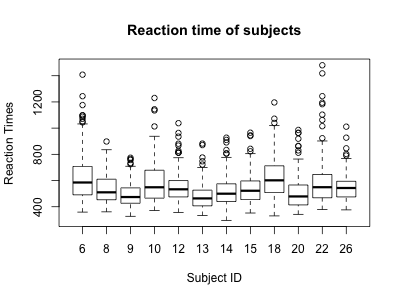
\includegraphics[scale=0.65]{figures/rxntime-boxplots.png}
  \end{center}

\end{frame}


%%%%%%%%%%%%%%%%%%%%%%%%%%%%%%%%%%%

\begin{frame}[fragile]
  \frametitle{ANOVA Review}

Number of observations $n = 1920$.

\hfill \\

{\footnotesize
\begin{tabular}{lrrrrr}
  \hline
 & Df & Sum Sq & Mean Sq & F value & Pr($>$F) \\ 
  \hline
rxntime\$Subject & ?? & 4060822.10 & 369165.65 & 20.05 & 0.0000 \\ 
  Residuals & ?? & 35129401.48 & 18411.64 &  &  \\ 
   \hline
\end{tabular}
}

% Response: PictureTarget.RT
%                      Df   Sum Sq Mean Sq F value    Pr(>F)    
% as.factor(Subject)   11  4060822  369166  20.051 < 2.2e-16 ***
% Residuals          1908 35129401   18412 

\clicker{What are the degrees of freedom?}
\begin{enumerate}[(a)]
\item  1 and 1909
\item \solnMult{11 and 1908}
\item 11 and 1909
\item 12 and 1908
\end{enumerate}

\end{frame}

%%%%%%%%%%%%%%%%%%%%%%%%%%%%%%%%%%%

\begin{frame}[fragile]
  \frametitle{ANOVA Review}

  (Assume $\alpha = 0.05$.)

  \clicker{What is the most appropriate conclusion?}
  \begin{enumerate}[(a)]
  \item There is no evidence that the subjects have different mean reaction times.
  \item There is no evidence that some of the subjects have the same mean reaction times.
  \item \solnMult{Some pairs of subjects have different mean reaction times.}
  \item All paris of subjects have different mean reaction times.
  \end{enumerate}

\end{frame}

%%%%%%%%%%%%%%%%%%%%%%%%%%%%%%%%%%%

\section{Main ideas}

%%%%%%%%%%%%%%%%%%%%%%%%%%%%%%%%%%%

\subsection{To identify which means are different, use pairwise t-tests}
\label{mi1}

%%%%%%%%%%%%%%%%%%%%%%%%%%%%%%%%%%%

\begin{frame}
\frametitle{Multiple testing}

\clicker{Suppose we want to determine which subjects have a mean reaction time different than Subject 6. How many pairwise t-tests will we need to do? Remember: there were a total of 12.}

\begin{enumerate}[(a)]
\item 6
\item \solnMult{11}
\item 12
\item $\frac{6 \times 5}{2} = 15$
\end{enumerate}

\end{frame}


%%%%%%%%%%%%%%%%%%%%%%%%%%%%%%%%%%%

\begin{frame}
\frametitle{Multiple testing}

\clicker{Suppose we want to determine which means are different from each other. How many pairwise t-tests would we need to conduct? Remember: there were a total of 12 groups.}

\begin{enumerate}[(a)]
\item 12
\item 12! = 479,001,600
\item $12 \times 11 = 132$
\item \solnMult{$\frac{12 \times 11}{2} = 66$}
\end{enumerate}

\end{frame}

%%%%%%%%%%%%%%%%%%%%%%%%%%%%%%%%%%%

\subsection{If you want to test many hypotheses simultaneously, use the Bonferroni correction}
\label{mi2}

%%%%%%%%%%%%%%%%%%%%%%%%%%%%%%%%%%%

\begin{frame}
  \frametitle{2. If you want to test many hypotheses simultaneously, use the Bonferroni correction}

\vfill

Bonferroni correction: 
\begin{itemize}
\item Target type I error rate: $\alpha$.

\item Number of null/alt hypotheses to be tested using the same data set: $K$

\item If you set the significance level for each test to be
\[
\alpha^* = \alpha / K,
\]
then the probability of making one or more type I errors is $ \leq \alpha$.

\end{itemize}

\vfill

\end{frame}

%%%%%%%%%%%%%%%%%%%%%%%%%%%%%%%%%%%

\begin{frame}
  \frametitle{}

\vfill

\app{4.6 ANOVA - Pt 2}{See the course webpage for details.}

\vfill

\end{frame}

%%%%%%%%%%%%%%%%%%%%%%%%%%%%%%%%%%%

\section{Summary}

%%%%%%%%%%%%%%%%%%%%%%%%%%%%%%%%%%%

\begin{frame}
\frametitle{Summary of main ideas}

\vfill

\begin{enumerate}

\item \nameref{mi1}

\item \nameref{mi2}

\end{enumerate}

\vfill

\end{frame}

%%%%%%%%%%%%%%%%%%%%%%%%%%%%%%%%%%%

\end{document}